\documentclass{article}
\usepackage[utf8]{inputenc}
\usepackage[english, ukrainian]{babel}
\usepackage{fontsize}
\usepackage{geometry}
\usepackage{amsthm}
\usepackage{amsfonts}
\usepackage{graphicx}
\usepackage[ruled]{algorithm2e}
\usepackage{hyperref}
\usepackage{biblatex}
\usepackage{csquotes}
\usepackage{mathtools}
\usepackage{amsmath}
\usepackage{amssymb}
\usepackage{bbm}
\usepackage{tabularx}
\usepackage{xcolor}

\usepackage{tikz}
\usetikzlibrary{decorations.pathmorphing}

\usepackage{enumitem}
\usepackage{nicefrac}

\usetikzlibrary{patterns}

\usepackage{diagbox}
\usepackage{longtable}

\usepackage{float}


\usepackage{enumitem}
\usepackage{nicefrac}

\usepackage{listings}
\definecolor{codegreen}{rgb}{0,0.6,0}
\definecolor{codegray}{rgb}{0.5,0.5,0.5}
\definecolor{codepurple}{rgb}{0.58,0,0.82}
\definecolor{backcolour}{rgb}{0.95,0.95,0.92}

\lstdefinestyle{mystyle}{
    backgroundcolor=\color{backcolour},   
    commentstyle=\color{codegreen},
    keywordstyle=\color{magenta},
    numberstyle=\tiny\color{codegray},
    stringstyle=\color{codepurple},
    basicstyle=\ttfamily\footnotesize,
    breakatwhitespace=false,         
    breaklines=true,                 
    captionpos=b,                    
    keepspaces=true,                 
    numbers=left,                    
    numbersep=5pt,                  
    showspaces=false,                
    showstringspaces=false,
    showtabs=false,                  
    tabsize=2
}

\lstset{style=mystyle}
\hypersetup{colorlinks=true, linkcolor=[RGB]{255, 3, 209}, citecolor={black}}

\graphicspath{ {../Images/} }

\begin{document}
    \begin{titlepage}
        \begin{center}
        $\newline$
        \vspace{3.3cm}
        
        {\LARGE\textbf{Лабораторна робота №4\\"Система прийняття рішень на основі нечітких правил для моделювання експертних систем"}}
        \vspace{10cm}
        \begin{flushright}
            \textbf{Роботу виконав:}\\Климентьєв Максим \\3-го курсу\\групи ФІ-21
        \end{flushright}
        \end{center}
    \end{titlepage}
    \newpage

    \pagenumbering{gobble}
    \tableofcontents
    \cleardoublepage
    \pagenumbering{arabic}
    \setcounter{page}{3}

    \newpage

    \section{Загальний опис задачі}
    Варіант 1: Вирішіть проблему контролера кондиціонера. Прикладом вхідних параметрів можуть бути “Температура”, “Вологість” та інше. Вихід: “Швидкість компресора”, “режим роботи”.
    
    \section{Опис усіх вхідних та вихідних параметрів}
    Вхідні параметри
    \begin{itemize}
        \item \textbf{Температура} --- Температура в кімнаті, в градусах Цельсія.
        \item \textbf{Вологість} --- Вологість в кімнаті, у відсотках.
        \item \textbf{Час} --- Час доби, у годинах.
    \end{itemize}

    Вихідні параметри
    \begin{itemize}
        \item \textbf{Швидкість компресора} --- Швидкість, у відсотках
        \item \textbf{Режим} --- Охолодження, підтримання або обігрівання
    \end{itemize}

    \section{Опис правил та функцій приналежності}
    \begin{itemize}
        \item Якщо температура cold, вологість low та час morning, то тоді швидкість компресора slow та режим роботи heating
        \item Якщо температура cold, вологість medium та час morning, то тоді швидкість компресора slow та режим роботи heating
        \item Якщо температура cold, вологість high та час morning, то тоді швидкість компресора medium та режим роботи heating
        \item Якщо температура normal, вологість low та час morning, то тоді швидкість компресора slow та режим роботи keeping
        \item Якщо температура normal, вологість medium та час morning, то тоді швидкість компресора medium та режим роботи keeping
        \item Якщо температура normal, вологість high та час morning, то тоді швидкість компресора fast та режим роботи keeping
        \item Якщо температура hot, вологість low та час morning, то тоді швидкість компресора medium та режим роботи cooling
        \item Якщо температура hot, вологість medium та час morning, то тоді швидкість компресора medium та режим роботи cooling
        \item Якщо температура hot, вологість high та час morning, то тоді швидкість компресора fast та режим роботи cooling
        \item Якщо температура cold, вологість low та час afternoon, то тоді швидкість компресора slow та режим роботи heating
        \item Якщо температура cold, вологість medium та час afternoon, то тоді швидкість компресора medium та режим роботи heating
        \item Якщо температура cold, вологість high та час afternoon, то тоді швидкість компресора fast та режим роботи heating
        \item Якщо температура normal, вологість low та час afternoon, то тоді швидкість компресора slow та режим роботи keeping
        \item Якщо температура normal, вологість medium та час afternoon, то тоді швидкість компресора medium та режим роботи keeping
        \item Якщо температура normal, вологість high та час afternoon, то тоді швидкість компресора fast та режим роботи keeping
        \item Якщо температура hot, вологість low та час afternoon, то тоді швидкість компресора slow та режим роботи cooling
        \item Якщо температура hot, вологість medium та час afternoon, то тоді швидкість компресора medium та режим роботи cooling
        \item Якщо температура hot, вологість high та час afternoon, то тоді швидкість компресора fast та режим роботи cooling
        \item Якщо температура cold, вологість low та час evening, то тоді швидкість компресора medium та режим роботи heating
        \item Якщо температура cold, вологість medium та час evening, то тоді швидкість компресора medium та режим роботи heating
        \item Якщо температура cold, вологість high та час evening, то тоді швидкість компресора fast та режим роботи heating
        \item Якщо температура normal, вологість low та час evening, то тоді швидкість компресора slow та режим роботи keeping
        \item Якщо температура normal, вологість medium та час evening, то тоді швидкість компресора medium та режим роботи keeping
        \item Якщо температура normal, вологість high та час evening, то тоді швидкість компресора fast та режим роботи keeping
        \item Якщо температура hot, вологість low та час evening, то тоді швидкість компресора slow та режим роботи cooling
        \item Якщо температура hot, вологість medium та час evening, то тоді швидкість компресора slow та режим роботи cooling
        \item Якщо температура hot, вологість high та час evening, то тоді швидкість компресора medium та режим роботи cooling
    \end{itemize}

    \begin{figure}[H]
        \centering
        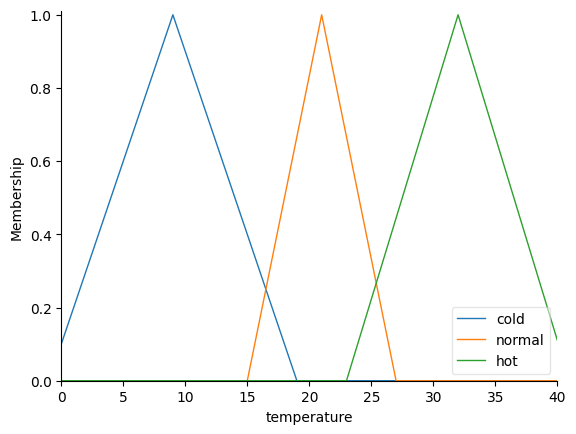
\includegraphics[width=0.6\linewidth]{temperature.png}
    \end{figure}

    \begin{figure}[H]
        \centering
        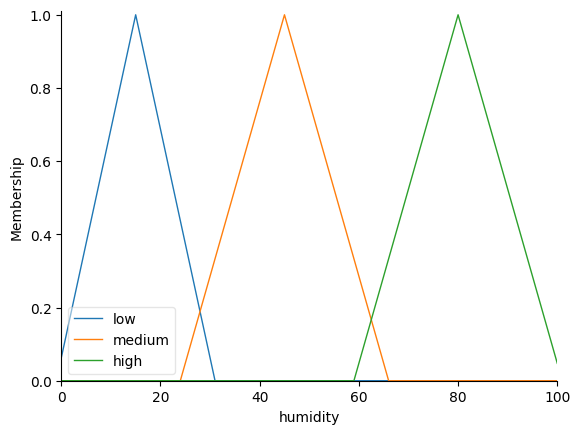
\includegraphics[width=0.6\linewidth]{humidity.png}
    \end{figure}
    
    \begin{figure}[H]
        \centering
        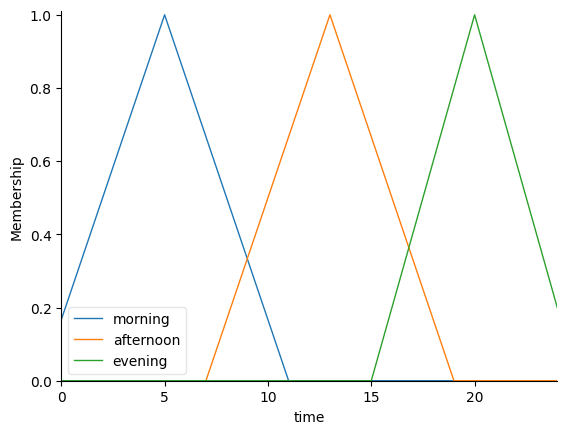
\includegraphics[width=0.6\linewidth]{time.png}
    \end{figure}

    \begin{figure}[H]
        \centering
        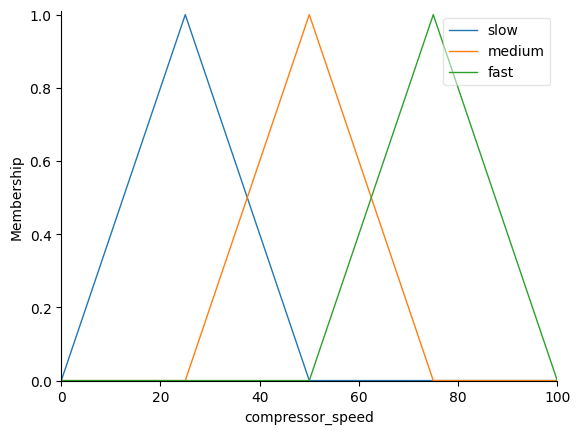
\includegraphics[width=0.6\linewidth]{compressor_speed.png}
    \end{figure}

    \begin{figure}[H]
        \centering
        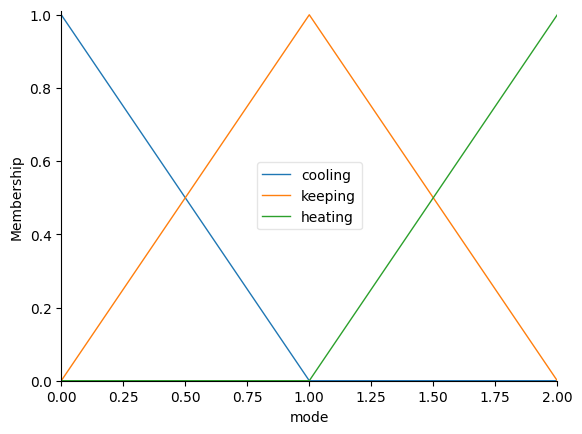
\includegraphics[width=0.6\linewidth]{mode.png}
    \end{figure}


    \section{Результати для кожного набору вхідних параметрів}

    На вхід прийшло: OrderedDict({'temperature': 1, 'humidity': 1, 'time': 1}) \\
    Швидкість компресора: 25.000000000000007 $ \approx $ slow \\
    Режим роботи: 1.5305555555555554 $ \approx $ heating \\

    На вхід прийшло: OrderedDict({'temperature': 38, 'humidity': 98, 'time': 22}) \\
    Швидкість компресора: 49.99999999999997 $ \approx $ medium \\
    Режим роботи: 0.4652014652014651 $ \approx $ cooling \\

    На вхід прийшло: OrderedDict({'temperature': 0, 'humidity': 0, 'time': 0}) \\
    Швидкість компресора: 25.0 $ \approx $ slow \\
    Режим роботи: 1.5154569892473118 $ \approx $ heating \\

    На вхід прийшло: OrderedDict({'temperature': 39, 'humidity': 99, 'time': 23}) \\
    Швидкість компресора: 49.99999999999999 $ \approx $ medium \\
    Режим роботи: 0.4765873015873016 $ \approx $ cooling \\

    На вхід прийшло: OrderedDict({'temperature': 40, 'humidity': 100, 'time': 24}) \\
    Швидкість компресора: 49.99999999999998 $ \approx $ medium \\
    Режим роботи: 0.4881920247773906 $ \approx $ cooling \\

    На вхід прийшло: OrderedDict({'temperature': 27.92, 'humidity': 50.54, 'time': 17.25}) \\
    Швидкість компресора: 34.983540750546965 $ \approx $ medium \\
    Режим роботи: 0.39838709677419354 $ \approx $ cooling \\
    
    \section{Висновки}
        Нечітку логіку задає людина, для того, аби їй самій потім не треба було руками перемикати параметри певного механізму.

        Нечітка логіка корисна для автоматизації, де не вистачає просто увімкнути чи вимкнути пристрій. Вона дає наближені, але цілком придатні результати.
    
        \subsection{Додатково бажано включити приклади задач, для яких нечітка логіка є придатною (свої приклади)}
            \begin{itemize}
                \item Розкладання та складання крил літаків залежно від швидкості літака.
                \item Паркування автомобіля залежно від відстані до кінця.
            \end{itemize}
        
\end{document}